\section{\textit{Sitemap}}

\subsection{Inleiding}

Die \textit{sitemap} is 'n visuele voorstelling van die struktuur van die
web- en mobiele toepassing. Dit bied 'n duidelike en georganiseerde
voorstelling van die verskillende bladsye en hul onderlinge navigasie verhoudings. Die
sitemap help om die navigasie en gebruikerservaring te verbeter deur 'n
duidelike hi\"erargie en struktuur te skep. Dit is 'n noodsaaklike element in die
ontwikkeling van die stelsel, aangesien dit die grondslag l\^e vir die
gebruikerskoppelvlak en die interaksies tussen verskillende bladsye.


\subsection{Administrasietoepassing \textit{sitemap}}
\begin{figure}[p]
    \centering
    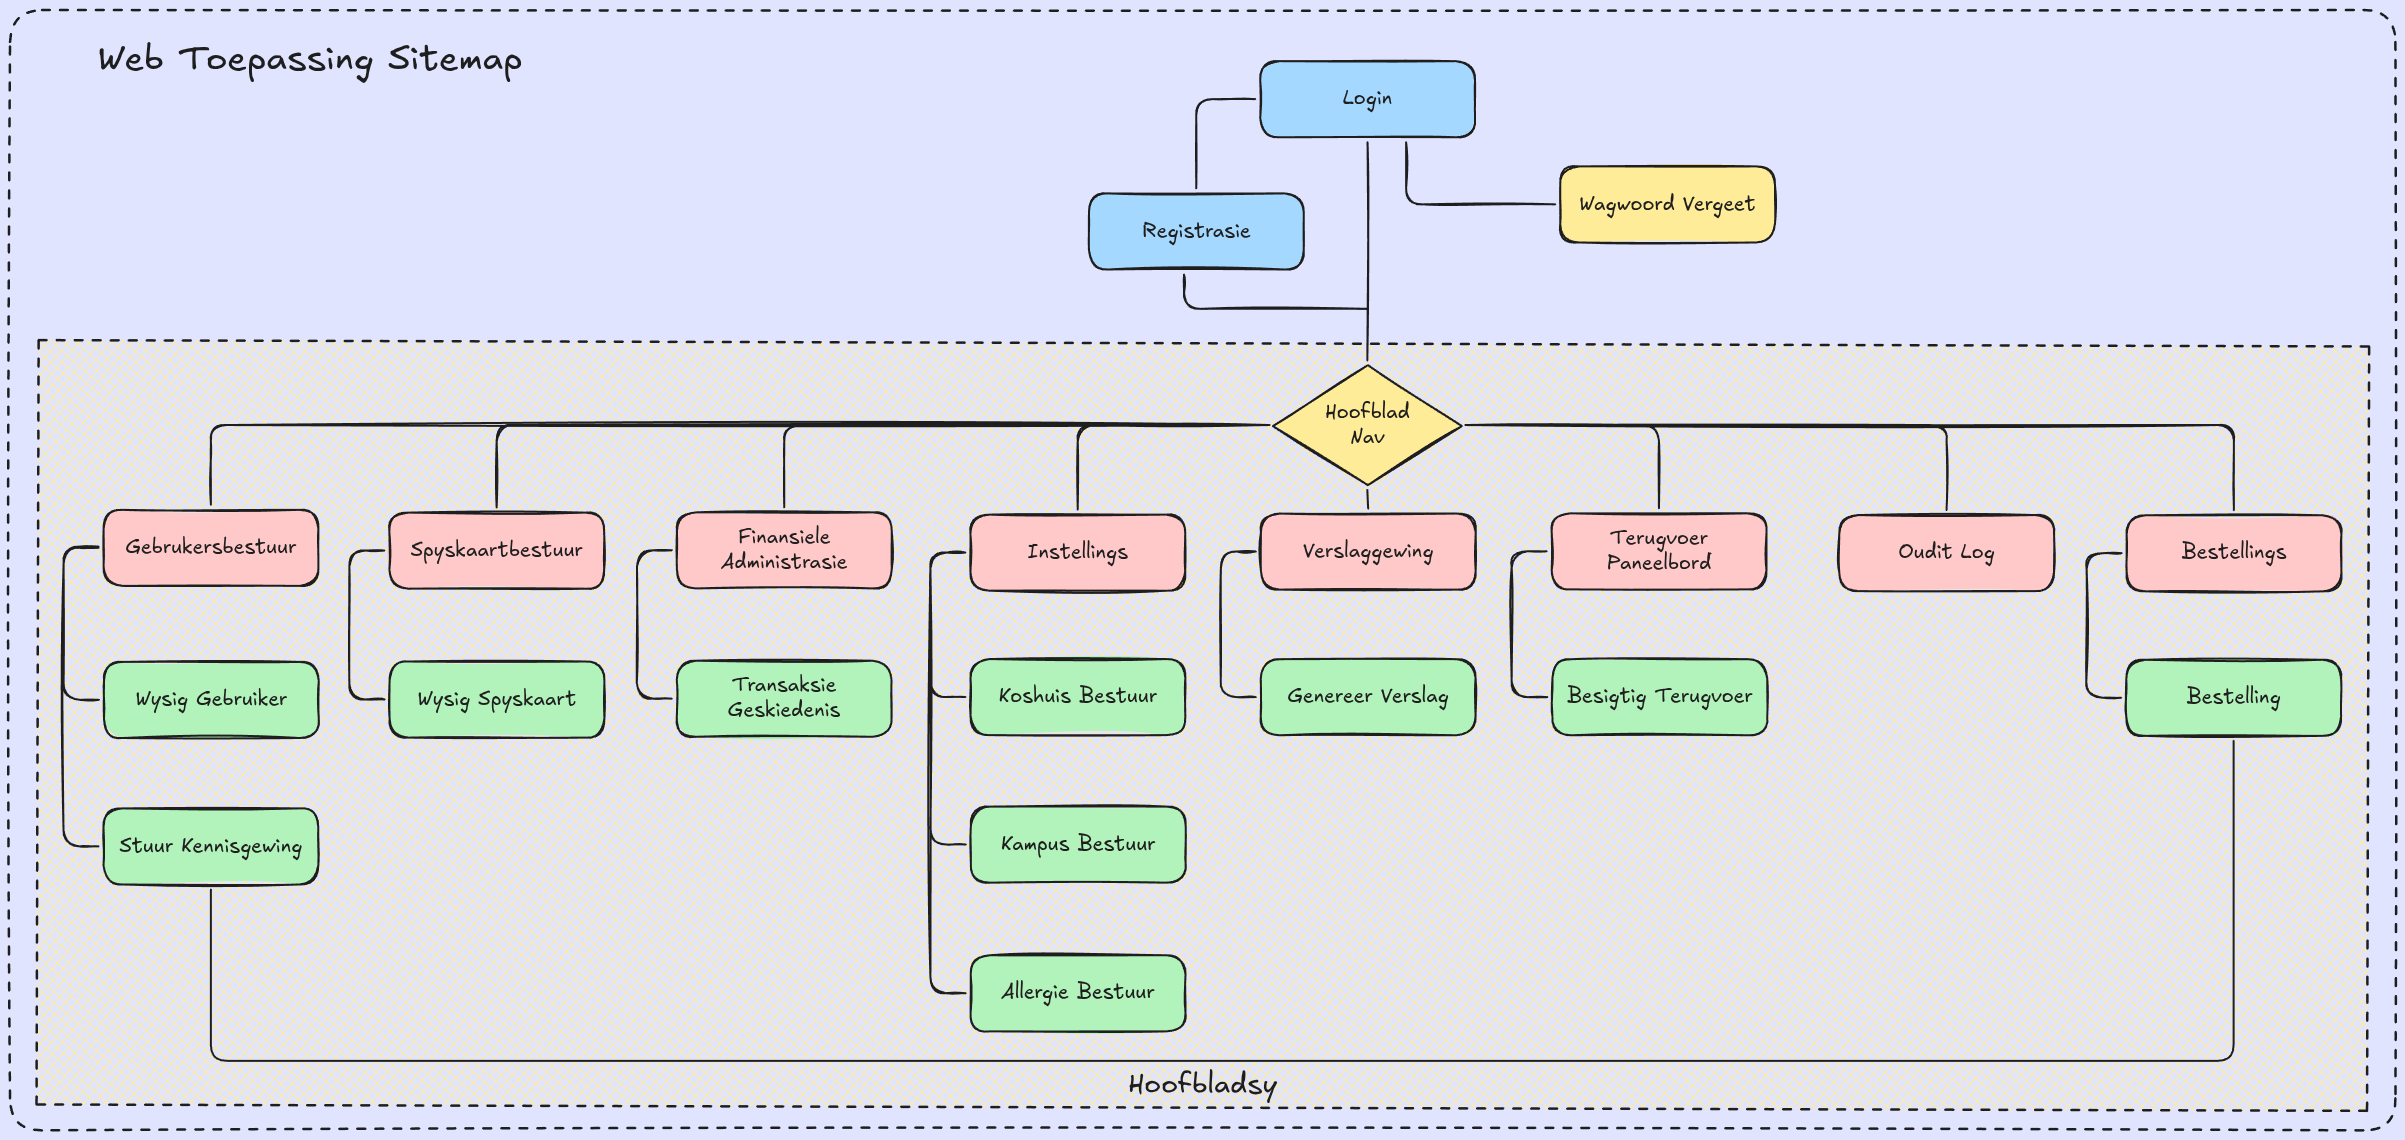
\includegraphics[width=0.9\textheight, angle=90]{figures/sitemap/admin.png}
    \caption{Sitemap vir die Administrasie Webplatform}
    \label{fig:admin_sitemap}
\end{figure}

Die beginpunt van die administrasietoepassing is die intekeningskerm, waar administrateurs kan inteken met hul
e-pos en wagwoord. Sodra hulle ingeteken is, word hulle na die hoofblad geneem,
waar hulle, volgens die administrateur se rolle, na die toepaslike paneelbord verwys word. Die paneelbord bied toegang tot verskeie funksies, afhangend van die
administrateur se rolle, soos gebruikersbestuur, spyskaartbestuur, finans\"iele
bestuur, instellings, verslaggewing, ouditlog en bestellings. Dit word aangedui
deur die hoofbladsy in die \textit{sitemap}, wat aangedui word as 'n samevoeging
van die verskillende paneelbord funksies.

Indien die administrateur toegang het tot die gebruikersbestuur, kan hulle
gebruikers wysig, skep, of verwyder. Hulle kan ook gebruikersrolle wysig en
kennisgewings stuur.

Die spyskaartbestuurfunksie laat administrateurs toe om spyskaartitems te
skep, wysig of verwyder. Dit sluit die vermo\"e in om beskikbare items te skep en bestuur, en om bestel-, wysigingsperdatums en aflewerings te
stel vir spesifieke items.

Die finans\"iele bestuurfunksie laat administrateurs toe om transaksies te
besigtig, gebruikers se balanse te bestuur en krediet in gebruikersrekeninge
individueel of in bondels by te voeg.

Die instellingsbladsy laat administrateurs toe om algemene instellings van die
toepassing te bestuur, soos die koshuis-, kampus- en allergenelys.

Die verslaggewingsfunksie bied administrateurs die vermo\"e om verslae te
genereer oor gebruikersaktiwiteite, bestellings en finansies.

Die terugvoerfunksie laat administrateurs toe om terugvoer van gebruikers te
besigtig en te bestuur. Dit sluit die vermo\"e in om terugvoer te filter en
te sorteer, en om terugvoer per e-pos op te volg.

Die ouditlogfunksie bied 'n gedetailleerde rekord van alle
administrasie-aktiwiteite, insluitend gebruikersaktiwiteite, stelselveranderings
en foutopsporing. Dit help om die stelsel se sekuriteit en integriteit te
verseker.

Die bestellingsbladsy laat administrateurs toe om bestellings te besigtig,
te bestuur en te verwerk. Dit sluit die vermo\"e in om bestellings te filter en
te sorteer, en om bestellingsstatusse te wysig.

\subsection{Gebruikertoepassing \textit{sitemap}}
\begin{figure}[H]
    \centering
    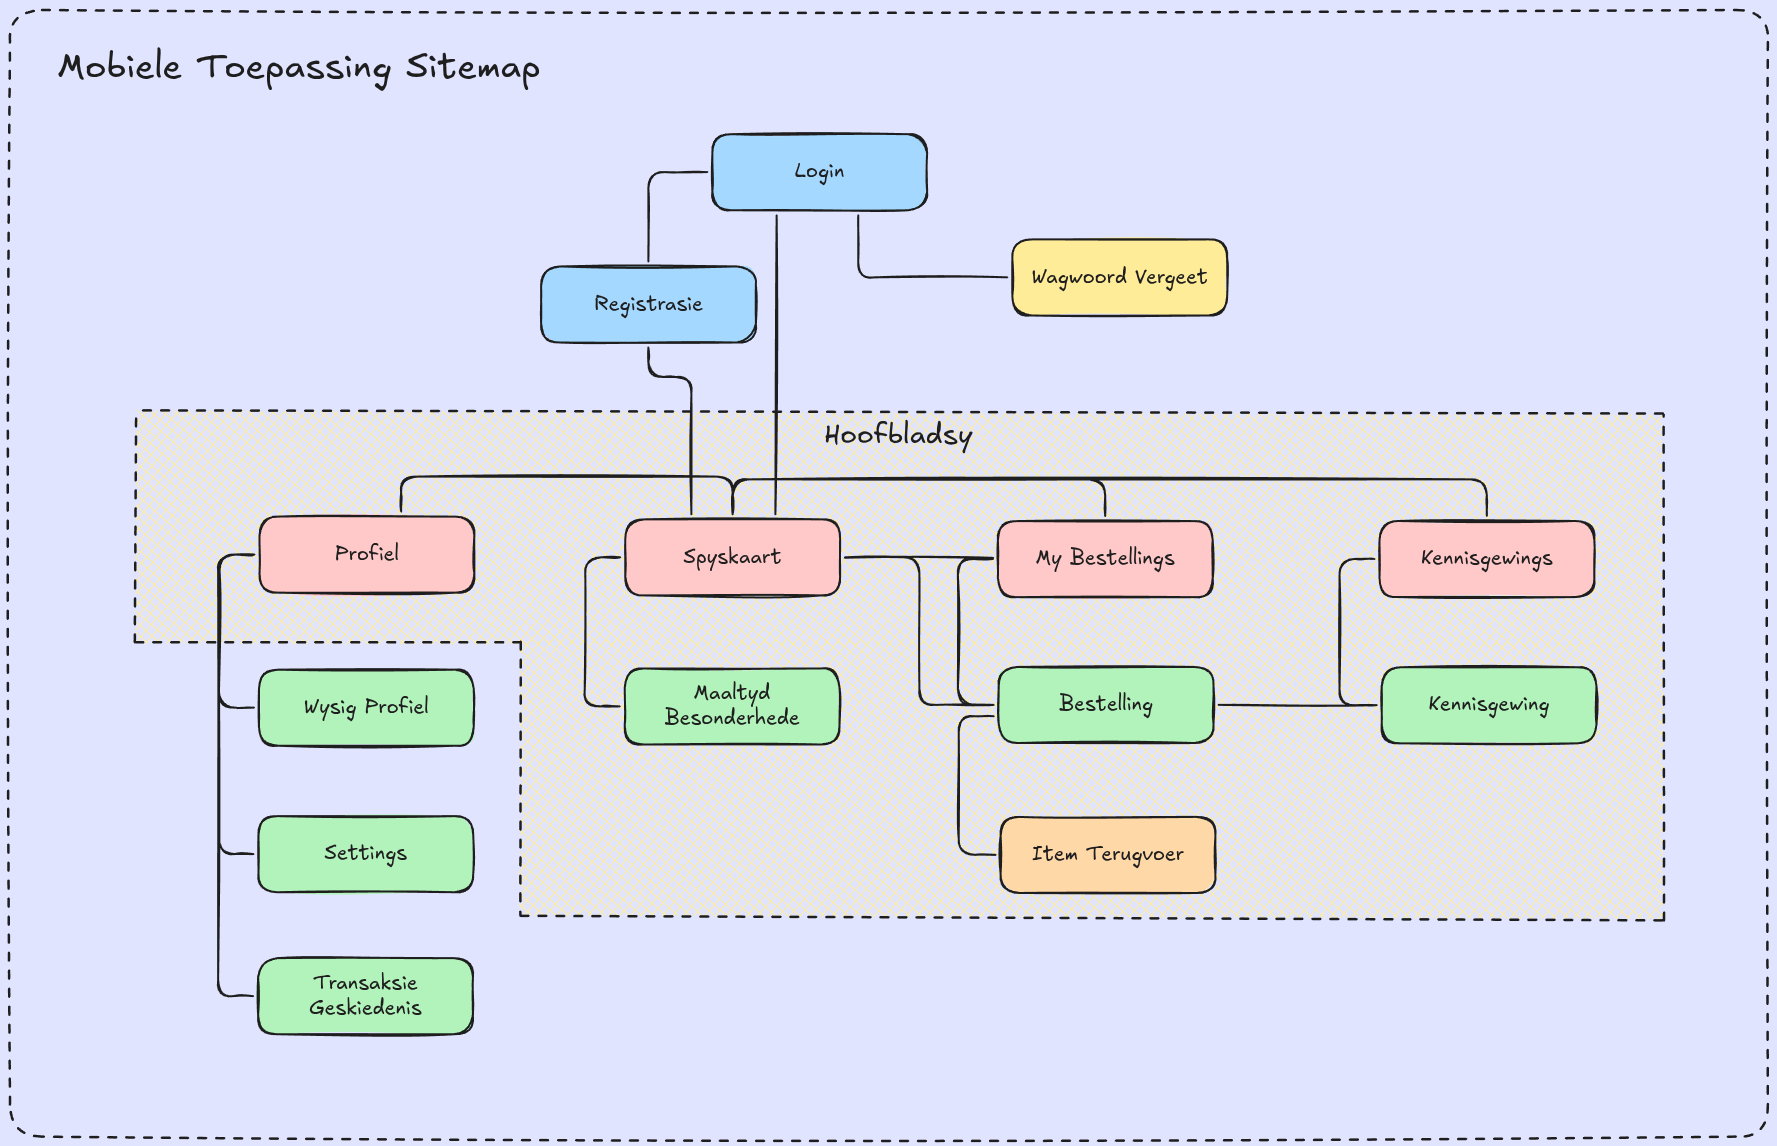
\includegraphics[width=0.9\textheight, angle=90]{figures/sitemap/mobile.png}
    \caption{Sitemap vir die Gebruiker Webplatform}
    \label{fig:user_sitemap}
\end{figure}

Die beginpunt van die gebruikertoepassing is die intekeningskerm, waar gebruikers kan inteken met hul e-pos en
wagwoord. Sodra hulle ingeteken is, word hulle na die hoofblad geneem, waar hulle
toegang het tot verskeie funksies soos die spyskaart, bestellings en terugvoer.

Die gebruiker het ook die vermo\"e om 'n nuwe gebruiker te skep deur die
registrasie skakel te volg. Dit sluit die invoer van persoonlike inligting soos
naam, van, e-pos en wagwoord in, verder word die gebruiker gevra in 'n
adisisonele vorm om hul student- of personeelnommer, koshuis, kampusligging en allergene te spesifiseer.

Die spyskaartbladsy bied 'n lys van beskikbare items wat gebruikers kan
besigtig en bestel. Gebruikers kan items bestel deur uit die beskikbare items te
kies en die verlangde hoeveelheid te spesifiseer.

Die bestellingsbladsy laat gebruikers toe om hul bestaande en vorige
bestellings te besigtig, te bestuur en te volg. Dit sluit die vermo\"e in om
bestellings te filter en te sorteer, en terugvoer oor bestellings te lewer.

Die kennisgewingsbladsy bied gebruikers die vermo\"e om kennisgewings te
besigtig en te bestuur. Dit sluit die vermo\"e in om kennisgewings te lees en
te verwyder, en om aksies op kennisgewings te neem, soos om 'n bestelling te
besigtig.

Die profielbladsy laat gebruikers toe om hul profiel te besigtig en te wysig.
Dit sluit die vermo\"e in om hul persoonlike inligting, soos naam, van, e-pos,
wagwoord, kampusligging, koshuis en allergene, te wysig. Gebruikers kan ook hul
kennisgewingvoorkeure wysig. Verder kan gebruikers hul transaksiegeskiedenis
besigtig en hul balans en krediet te besigtig.
